\documentclass{article}

\usepackage{caption}
\usepackage{subcaption}
\usepackage{graphicx}
\usepackage{tikz}
\usepackage{tikzsymbols}
\usetikzlibrary{calc}
\usepackage{float}
\usepackage{pdflscape}
\usepackage{geometry}
\geometry{a4paper, landscape, margin=1cm}


\def\centerarc[#1](#2)(#3:#4:#5){\draw[#1] ($(#2)+({#5*cos(#3)},{#5*sin(#3)})$) arc (#3:#4:#5);}



\pagestyle{empty}
\begin{document}
	\centering
	\begin{figure}[H]
		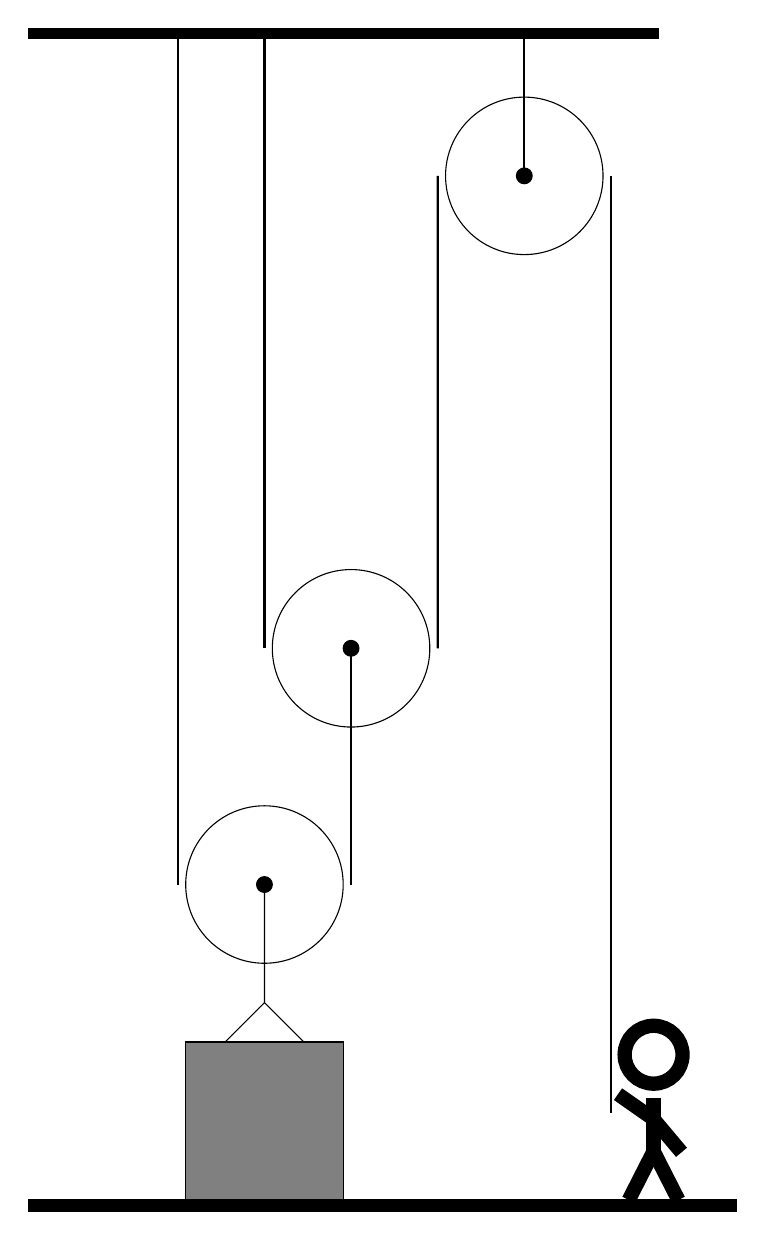
\begin{tikzpicture}
			%%%%% START %%%%%
			\def\a{11.75}
			\def\radlg{1}
			\def\radrp{1.1}
			\def\radsm{0.1}
			\def\yone{1}
			\def\xone{1}
			\def\ytwo{10}
			\def\xtwo{3.2}
			\def\xthree{2.1}
			\def\ythree{4}
			\def\xfour{4.3}
			\def\dx{5.9}
			\def\dy{-1.9}
			\def\dw{1.75mm}
			
			\draw[fill=black] (-2,\a) rectangle (6,\a+0.125);
			
			\draw (\xone,\yone) circle (\radlg);
			\draw[fill=black] (\xone,\yone) circle (\radsm);
			
			\draw (\xthree,\ythree) circle (\radlg);
			\draw[fill=black] (\xthree,\ythree) circle (\radsm);
			
			\draw (\xfour,\ytwo) circle (\radlg);
			\draw[fill=black] (\xfour,\ytwo) circle (\radsm);
			\draw[thick] (\xfour,\ytwo) -- (\xfour,\a);
			
			\draw (\xone,\yone) -- (\xone,\yone-1.5) -- (\xone-0.5,\yone-2) -- (\xone+0.5,\yone-2) -- (\xone,\yone-1.5);
			\draw[fill=black!50] (\xone-1,\yone-2) rectangle (\xone+1,\yone-4); 
			
			\draw[thick] (\xone-\radrp,\a) -- (\xone-\radrp,\yone); 
			\centerarc[thick](\xone,\yone)(180:360:\radrp);
			\draw[thick](\xone+\radrp,\yone) -- (\xthree,\ythree);
			\draw[thick] (\xthree-\radrp,\a) -- (\xthree-\radrp,\ythree);
			\centerarc[thick](\xthree,\ythree)(180:360:\radrp);
			\draw[thick](\xthree+\radrp,\ythree) -- (\xfour-\radrp,\ytwo);
			\centerarc[thick](\xfour,\ytwo)(0:180:\radrp);
			\draw[thick] (\xfour+\radrp,\ytwo) -- (\xfour+\radrp,-1.9);
%			\draw[line width=\dw] (\dx,\dy) circle (0.375);
%			\draw[line width=\dw] (\dx,\dy-0.375-0.15) -- (\dx,\dy-0.375-0.9);
%			\draw[line width=\dw] (\dx,\dy-0.375-0.9) -- (\dx-0.4,\dy-0.375-1.35);
%			\draw[line width=\dw] (\dx,\dy-0.375-0.9) -- (\dx+0.4,\dy-0.375-1.35);
%			\draw[line width=\dw] (\dx,\dy-0.375-0.5) -- (\dx-0.45,\dy-0.6);
%			\draw[line width=\dw] (\dx,\dy-0.375-0.5) -- (\dx+0.45,\dy-1.3);

			\node at (\dx,\dy) {\Strichmaxerl[10][-35][-50]};
			
			\draw[fill=black] (-2,-3) rectangle (7,-3.15);
			%%%%% END %%%%%
		\end{tikzpicture}
	\end{figure}
	
\end{document}